\section{Základy lineárního programování}

\begin{pozadavky}
\begin{pitemize}
	\item Simplexová metoda
	\item Věty o dualitě (bez důkazu)
\end{pitemize}
\end{pozadavky}

\ramcek{14cm}{Lineární programování je označení pro úlohu maximalizovat jistou funkci $n$ reálných proměnných na množině bodů polytopu v prostoru $\mathbb{R}^n$.}

Nejprve si udělejme malý výlet do geometrie. {\it Polytop} je zobecněním polygonu
(mnohoúhelníku) do vyšších dimenzích. Pro dimenzi $3$ se ale používá ještě speciální
název {\it polyhedron} a pro dimenzi $4$ {\it polychoron}. My se v dalším textu
omezíme na {\it konvexní polytopy}, což jsou konvexní obaly konečně mnoha bodů.
Vzhledem k tomu, že tyto konvexní polytopy jsou průnikem jistého množství poloprostorů,
můžeme je popsat maticovou rovnicí tvaru \[Ax\leq b,\] kde $A$ je matice řádu $m\times n$
a $m$ je počet poloprostorů, jejichž průnikem je daný polytop,
a $n$ je dimenze podprostoru, ve kterém polytop máme.

{\it Simplex} je \uv{$n$--dimenzionální} trojúhelník (průnik několika poloprostorů). Podle rostoucí dimenze je to tedy po řadě bod, úsečka, trojúhelník, čtyřstěn, pentachoron (viz obrázek 1) atd. Může být omezený i neomezený.

\begin{figure}[h]
\label{obr1}
\begin{center}
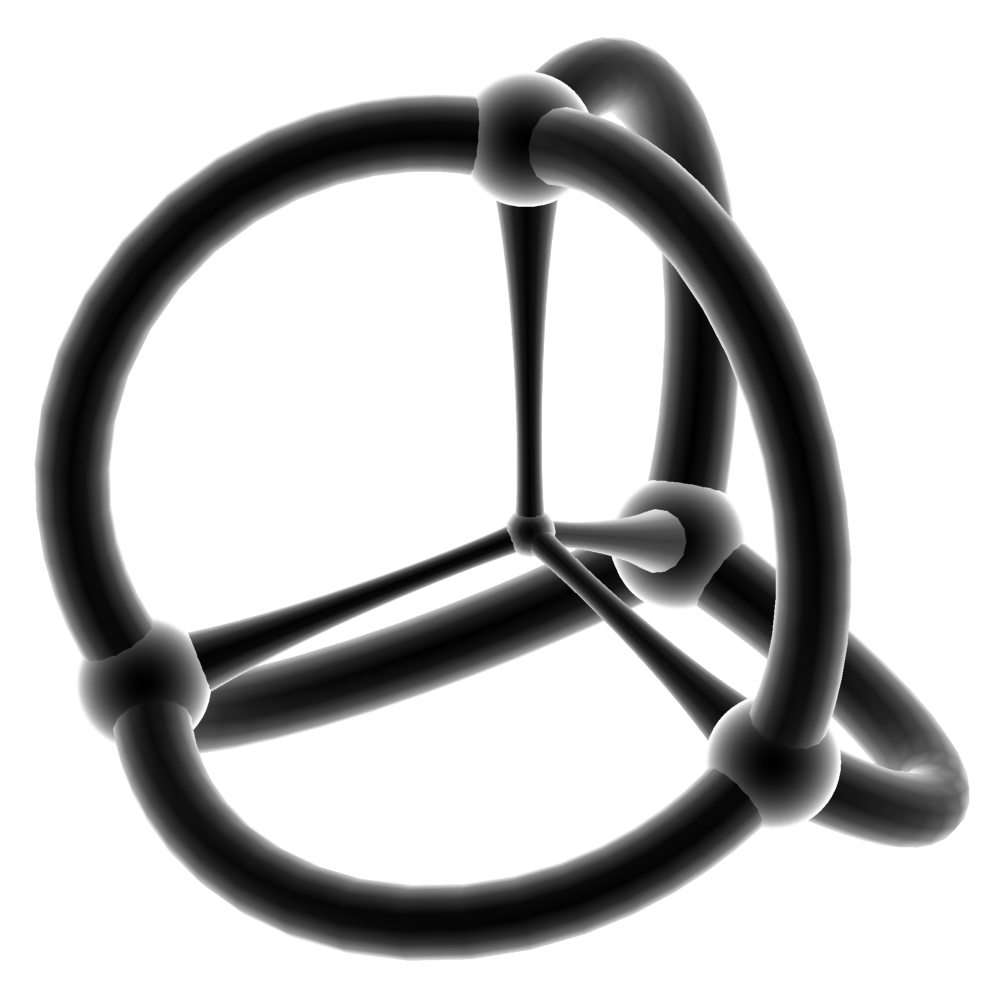
\includegraphics[width=4cm]{matematika/obrazky/4simplex.png}
\caption{Pentachoron}
\end{center}
\end{figure}

Nyní přistupme k formální definici úlohy lineárního programování.

\medskip
\ramcek{14cm}{
\noindent{\bf\textsf{Úloha lineárního programování}} \\
Je dán konvexní polytop v prostoru $\mathbb{R}^n$ popsaný $m$ nerovnostmi.
Maticově to můžeme zapsat ve tvaru $Ax\leq b$, kde $A$ je reálná matice
řádu $m\times n$ a $b$ je vektor $m$ reálných čísel. Dále je dán vektor
$c\in\mathbb{R}^n$. Funkce, kterou chceme maximalizovat, je $\sum_{i=1}^n c_ix_i$,
neboli vektorově $c^Tx$.
Ještě navíc hledáme pouze mezi body se všemi souřadnicemi
nezápornými (tj. $x_i\geq 0$ pro $i=1,\dots, n$).
}

\noindent\textsf{Terminologie}
\begin{penumerate}
 \item Vektoru $c$ říkáme {\it cenový vektor}, funkci $c^Tx$ pak {\it účelová funkce}.
 \item Nerovnosti $Ax\leq b$ a $x\geq 0$ jsou {\it omezující podmínky}, vektor $b$ je {\it pravá strana úlohy}.
 \item Konkrétní zadání úlohy lineárního programování (tj. matice $A$ a vektory $b$, $c$) je {\it přípustné},
pokud existuje nějaký bod splňující $x\geq 0$ a $Ax\leq b$. Jinak je zadání {\it nepřípustné}.
 \item Úloha je {\it neomezená}, pokud můžeme účelovou funkcí dosáhnout na přípustných bodech libovolně veliké hodnoty.
Jinak je {\it omezená}.
\end{penumerate}

\begin{veta}
Pro přípustnou a omezenou úlohu lineárního programování\,\footnote{Tedy existuje alespoň jedno řešení
a účelová funkce je shora omezená.} existuje bod, ve kterém účelová funkce nabývá maxima. Těchto
bodů obecně může být více a říkáme jim optimální řešení.
\end{veta}

\subsection{Simplexová metoda}

Simplexová metoda je označení pro algoritmus řešící úlohu lineárního programování. Byla publikována
v roce 1947 jedním ze zakladatelů lineárního programování američanem Georgem Dantzigem.

\medskip
\begin{center}
{\bf\textsf{Idea}}
\end{center}
\ramcek{14cm}{
Zkonstruujeme přípustné řešení v některém vrcholu polytopu. Poté jdeme po hranách do vrcholů
s vyšší hodnotou účelové funkce.}

Omezující podmínku $Ax\leq b$ tedy změníme na $Ax=b$. Toho docílíme přidáním jedné nezáporné proměnné pro každou podmínku ( $\sum{x}<b$ je totiž ekvivalentní $\sum{x}+y=b$ kde $y\in\mathbb{R}^+$). Tuto úpravu lze také zapsat jako $A:=(A\ I)$. Dále předpokládáme, že matice $A$ má lineárně nezávislé řádky.
Pro podmnožinu indexů $I\subseteq \{1, 2, \dots, n\}$
označme $A_I$ matici $A$, ze které ponecháme pouze sloupce, které jsou v~$I$. Analogicky pro libovolný vektor $w\in\mathbb{R}^n$
označme jako $w_I$ vektor, z něhož ponecháme jenom souřadnice z~$I$ (má dimenzi $n-|I|$).

\ramcek{14cm}{
{\it Báze} (a to nemá nic společného s bází vektorového prostoru) je libovolná podmnožina indexů $B\subseteq \{1, 2, \dots, n\}$ taková, že matice $A_B$ je regulární.
Navíc řekneme, že báze je {\it přípustná}, pokud rovnice $A_Bx_B=b$ má nezáporné řešení.
Vektor $x\in\mathbb{R}^n$ je tzv. {\it bazické řešení}\,\footnote{Někdy též bázové řešení.}, pokud existuje báze $B$ taková, že
$A_Bx_B=b$ a $x_i=0$ pro každé $i\in\{1,2,\dots,m\}\backslash B$.
}
Poznamenejme jen, že bazické řešení ještě nemusí být přípustné. Je-li navíc i přípustné,
říkáme mu přirozeně {\it přípustné bazické řešení}. Proměnným $x_j$ pro $j\in B$, kde
$B$ je báze, říkáme bazické.

\begin{veta}
Nechť $x\in\mathbb{R}^n$ je přípustné řešení. Pak $x$ je bazické řešení, právě když
sloupce matice $A$ odpovídající kladným proměnným jsou lineárně nezávislé.
\end{veta}
%\begin{dukaz}
%Jako $K$ označme množinu těch indexů, pro které je $x_j>0$. Implikace $\Rightarrow$ je jednoduchá,
%neboť je-li $x$ bazické řešení, pak existuje báze $B$ tak, že $A_B$ je regulární a $x_{[n]\backslash B}=0$.
%Jelikož jsou ale všechny souřadnice $x$ vně $B$ nulové, je nutně $K\subseteq B$, a tedy $A_K$ je rovněž regulární.
%Nyní ukažme implikaci $\Leftarrow$.
%\end{dukaz}

\begin{veta}
Nechť $B$ je $m$--prvková indexová množina $B\subseteq \{1,\dots, n\}$ a $A_B$ je regulární. Pak existuje
nejvýše jedno přípustné bazické řešení $x$ ($x_i\neq 0 \Leftrightarrow i\in B$).
\end{veta}

Mezi první tvrzeními jsme uvedli, že má-li daná úloha lineárního programování nějaké přípustné
řešení a je-li zároveň účelová funkce na množině přípustných řešení omezená, pak existuje
optimální řešení (tj. nabývá se maxima). Dá se ale dokázat dokonce následující.

\ramcek{14cm}{
\begin{veta}
Má-li daná úloha optimální řešení, pak i některé bazické řešení je optimální.
\end{veta}}
Tato věta má obrovskou důležitost, neboť je jasné, že {\bf bazických řešení je jen konečně mnoho}.
Ukažme si fungování simplexové metody na konkrétním příkladu.
\begin{priklad}
Maximalizujte funkci $z(x_1,\dots,x_5) = x_1+x_2$ za omezujících podmínek $x_i\geq 0$ ($i=1,\dots, 5$) a
\begin{center}
\fbox{
\begin{tabular}{rrrrrl}
$-x_1$ & $+x_2$ & $+x_3$ & & & $=1$     \\
$+x_1$ & & & $+x_4$ &  & $=3$       \\
& $+x_2$ & & & $+x_5$ & $=2$       \\
\end{tabular}}
\end{center}
\end{priklad}

\begin{proof}[Řešení]
Nejprve najdeme libovolné přípustné bazické řešení. Matice $A$ a vektor $b$ této úlohy jsou ze zadání
\[
A=
\left(
\begin{array}[h]{ccccc}
-1 & 1 & 1 & 0 & 0      \\
1 & 0 & 0 & 1 & 0       \\
0 & 1 & 0 & 0 & 1
\end{array}\right),\quad
b=\left(\begin{array}[h]{c}
   1 \\ 3 \\ 2
  \end{array}\right)
\]
a $m=3, n=5$. Vidíme tedy, že jedním z bazických řešení je $R_1 = (0,0,1,3,2)^T$. Odpovídající
báze indexů je $B=\{3,4,5\}$ (matice $A_B$ je jednotková, a tedy regulární). Na základě tohoto
vytvoříme tzv. {\it simplexovou tabulku} (počáteční přípustnou tabulku) tak, že vyjádříme bazické proměnné
pomocí nebazických a přidáme jeden řádek s vyjádřenou účelovou funkcí pomocí nebazických proměnných.
\[
\begin{array}{c|ccc}
x_3=& 1 & +x_1 & -x_2   \\
x_4=& 3 & -x_1 &        \\
x_5=& 2 & & -x_2        \\
\hline
z=& & x_1 & +x_2
\end{array}, \quad R_1 = (0,0,1,3,2)^T, \quad z=0
\]

V bodě $R_1$ je $z(R_1) = 0$. Nyní budeme, jak bylo naznačeno, postupně zvyšovat
hodnotu funkce $z$, dokud nezjistíme, že jsme nalezli optimální řešení. Hodnotu funkce $z$ budeme
zvětšovat zvětšením hodnoty některé nebazické (volné) proměnné.

Ponechejme $x_1=0$ a zvětšeme $x_2$ z $0$ na $1$ (jednička je nejlepší možná, viz první rovnici a $x_3\geq 0$).
Pak pomocí tabulky dostaneme nové přípustné řešení, konkrétně $R_2=(0,1,0,3,1)^T$. Z první rovnice teď
vyjádříme $x_2$:
\[
x_2 = 1+x_1-x_3
\]
a nahradíme touto rovnicí původní první rovnici $x_3=1+x_1-x_2$. Toto řešení odpovídá bázi $B=\{2,4,5\}$.
Snadno zjistíme, že $z(R_2) = 0+1 = 1$. Nyní se stalo, že proměnná $x_2$ nahradila proměnnou $x_3$ v bázi.
Tomuto procesu říkáme, že proměnná $x_2$ \uv{vstoupila do báze}, $x_3$ z ní \uv{vystoupila}.
\smallskip

Dostáváme tak novou simplexovou tabulku
\[
\begin{array}{c|ccc}
x_2=& 1 & +x_1 & -x_3   \\
x_4=& 3 & -x_1 &        \\
x_5=& 1 & -x_1& +x_3        \\
\hline
z=& 1& +2x_1 & -x_3
\end{array}, \quad R_2=(0,1,0,3,1)^T, \quad z=1
\]
Nyní budeme zvyšovat $x_1$. První rovnice $x_1$ neomezuje, druhá říká $x_1\leq 3$ a třetí nyní říká $x_1\leq 1$
(jelikož $x_3=0$). Položme tedy $x_1=1$. Dostáváme nové řešení $R_3=(1,2,0,2,0)^T, z(R_3) = 3$. Proměnná
$x_1$ vstoupí do báze místo proměnná $x_5$. Nová báze je $B=\{1,2,4\}$.
\smallskip

Dostáváme další simplexovou tabulku
\[
\begin{array}{c|ccc}
x_1=& 1 & +x_3 & -x_5   \\
x_2=& 2 &  &  -x_5       \\
x_4=& 2 & -x_3& +x_5        \\
\hline
z=& 3& +x_3 & -2x_5
\end{array}, \quad R_3=(1,2,0,2,0)^T, \quad z=3
\]
Zvětšíme $x_3$ z $0$ na $2$ ($x_3\leq 2$ plyne ze třetí rovnice tabulky) a tím obdržíme
další řešení $R_4=(3,2,2,0,0)^T$, báze je $B=\{1,2,3\}$, $z(R_4)=5$. Odpovídající nová
simplexová tabulka je
\[
\begin{array}{c|ccc}
x_1=& 3 & -x_4 &    \\
x_2=& 2 &  &  -x_5       \\
x_3=& 2 & -x_4& +x_5        \\
\hline
z=& 5& -x_4 & -x_5
\end{array}, \quad R_4=(3,2,2,0,0)^T, \quad z=5
\]
Nyní je jasné, že libovolné zvýšení volné proměnné $x_4$ nebo $x_5$ sníží hodnotu účelové funkce.
Z konstrukce simplexové metody plyne, že řešení $R_4$ je již optimální, neboť jsme prováděli pouze
ekvivalentní rovnicové úpravy. Optimálním řešením dané úlohy je tedy bod $(3,2,2,0,0)$.



\end{proof}




Časová složitost simplexové metody je $O(2^n)$.
Jeden z nejhorších případů můžeme vzít $n$--dimenzionální krychli,
která má přesně $2^n$ vrcholů. Na této krychli algoritmus
může postupně navštívit všechny její vrcholy. 

Simplexová metoda nachází uplatnění převážně při řešení optimalizačních úloh v inženýrství nebo ekonomii.

\subsection{Duální úloha}

Problém lineárního programování tak, jak byl popsán výše, označujeme jako {\it primární}.
Ke každému primárnímu problému můžeme zkonstruovat {\it duální úlohu}. Připomeňme, že
primární úloha byla najít
\[
\max\{ c^Tx : x\in\mathbb{R}^n, Ax\leq b, x\geq 0 \}.
\]
Duální úloha k této pak je najít
\[
\min\{ b^Ty : y\in\mathbb{R}^m, A^Ty\geq c, y\geq 0 \}.
\]
Základem teorie duality lineárního programu jsou následující dvě věty -- {\it (Slabá) věta o dualitě}.

\begin{vetaN}{Slabá věta o dualitě}
Pokud je $x$ přípustné řešení primární úlohy a $y$ přípustné řešení duální úlohy, pak
hodnota duální účelové funkce v bodě $y$ je alespoň tak veliká jako hodnota primární účelové
funkce v bodě $x$.
\end{vetaN}

\begin{vetaN}{Věta o dualitě}
Nechť $x_*$ je optimální řešení primární úlohy. Pak existuje optimální řešení $y_*$ duální úlohy takové, že
\[
c^Tx_* = b^Ty_*.
\]
\end{vetaN}
\bigskip

\noindent{\bf\textsf{Duální úloha ze života}}

\dots 

%Mějme malou pekárničku na rohu ulice a školačku Kačenku, která si chce koupit
%něco dobrého ke~svačině. V pekárničce prodávají dva druhy zboží -- bábovky a pařížské dorty.
%Bábovka stojí 80 Kč, pařížský dort 50 Kč. Pekárníčku vlastní jedna hodná paní ze sousedství, a proto
%si můžete vzít i jen kousek bábovky nebo dortíku. Na pařížský dortík jsou potřeba
%3 unce čokolády, 2 unce cukru a 2 unce krému. Na bábovku pak jsou potřeba
%4 unce cukru a 5 uncí krému. Jelikož ale Kačenka dá na správnou výživu,\footnote{A daří se jí to převelice.}
%ví, že musí jíst hodnotně, a proto si stanovila, že chce, aby její svačinka měla alespoň 6
%uncí čokolády, 10 uncí cukru a 8 uncí krému. Jelikož má ale malinkatou peněženku, do které se jí
%nevešelo moc penízků, chce, aby si svačinku splňující daná kritéria nakoupila co nejlevněji.
%Pomůžete milé Kačence?
%\medskip


%Zaveďme nyní $m$ nových proměnných $x_{n+1}, x_{n+2}, \dots, x_{n+m}$ pomocí vztahu
%\[
%x_{n+i} = b_i - \sum_{j=1}^n A_{ij}x_j,\quad i=1, 2, \dots, m
%\]
%a přidejme pro každou takto nově vytvořenou proměnnou ještě omezující podmínku $x_{n+i}\geq 0$.
%Každá proměnná $x_{n+i}$ je tedy jakousi \uv{chybou} (rozdílem) hodnoty pravé strany
%a hodnoty levé strany $i$--té nerovnosti.
